%% Beginning of file 'sample631.tex'
%%
%% Modified 2021 March
%%
%% This is a sample manuscript marked up using the
%% AASTeX v6.31 LaTeX 2e macros.
%%
%% AASTeX is now based on Alexey Vikhlinin's emulateapj.cls 
%% (Copyright 2000-2015).  See the classfile for details.

%% AASTeX requires revtex4-1.cls and other external packages such as
%% latexsym, graphicx, amssymb, longtable, and epsf.  Note that as of 
%% Oct 2020, APS now uses revtex4.2e for its journals but remember that 
%% AASTeX v6+ still uses v4.1. All of these external packages should 
%% already be present in the modern TeX distributions but not always.
%% For example, revtex4.1 seems to be missing in the linux version of
%% TexLive 2020. One should be able to get all packages from www.ctan.org.
%% In particular, revtex v4.1 can be found at 
%% https://www.ctan.org/pkg/revtex4-1.

%% The first piece of markup in an AASTeX v6.x document is the \documentclass
%% command. LaTeX will ignore any data that comes before this command. The 
%% documentclass can take an optional argument to modify the output style.
%% The command below calls the preprint style which will produce a tightly 
%% typeset, one-column, single-spaced document.  It is the default and thus
%% does not need to be explicitly stated.
%%
%% using aastex version 6.3
\documentclass[linenumbers]{aastex631}

%% The default is a single spaced, 10 point font, single spaced article.
%% There are 5 other style options available via an optional argument. They
%% can be invoked like this:
%%
%% \documentclass[arguments]{aastex631}
%% 
%% where the layout options are:
%%
%%  twocolumn   : two text columns, 10 point font, single spaced article.
%%                This is the most compact and represent the final published
%%                derived PDF copy of the accepted manuscript from the publisher
%%  manuscript  : one text column, 12 point font, double spaced article.
%%  preprint    : one text column, 12 point font, single spaced article.  
%%  preprint2   : two text columns, 12 point font, single spaced article.
%%  modern      : a stylish, single text column, 12 point font, article with
%% 		  wider left and right margins. This uses the Daniel
%% 		  Foreman-Mackey and David Hogg design.
%%  RNAAS       : Supresses an abstract. Originally for RNAAS manuscripts 
%%                but now that abstracts are required this is obsolete for
%%                AAS Journals. Authors might need it for other reasons. DO NOT
%%                use \begin{abstract} and \end{abstract} with this style.
%%
%% Note that you can submit to the AAS Journals in any of these 6 styles.
%%
%% There are other optional arguments one can invoke to allow other stylistic
%% actions. The available options are:
%%
%%   astrosymb    : Loads Astrosymb font and define \astrocommands. 
%%   tighten      : Makes baselineskip slightly smaller, only works with 
%%                  the twocolumn substyle.
%%   times        : uses times font instead of the default
%%   linenumbers  : turn on lineno package.
%%   trackchanges : required to see the revision mark up and print its output
%%   longauthor   : Do not use the more compressed footnote style (default) for 
%%                  the author/collaboration/affiliations. Instead print all
%%                  affiliation information after each name. Creates a much 
%%                  longer author list but may be desirable for short 
%%                  author papers.
%% twocolappendix : make 2 column appendix.
%%   anonymous    : Do not show the authors, affiliations and acknowledgments 
%%                  for dual anonymous review.
%%
%% these can be used in any combination, e.g.
%%
%% \documentclass[twocolumn,linenumbers,trackchanges]{aastex631}
%%
%% AASTeX v6.* now includes \hyperref support. While we have built in specific
%% defaults into the classfile you can manually override them with the
%% \hypersetup command. For example,
%%
%% \hypersetup{linkcolor=red,citecolor=green,filecolor=cyan,urlcolor=magenta}
%%
%% will change the color of the internal links to red, the links to the
%% bibliography to green, the file links to cyan, and the external links to
%% magenta. Additional information on \hyperref options can be found here:
%% https://www.tug.org/applications/hyperref/manual.html#x1-40003
%%
%% Note that in v6.3 "bookmarks" has been changed to "true" in hyperref
%% to improve the accessibility of the compiled pdf file.
%%
%% If you want to create your own macros, you can do so
%% using \newcommand. Your macros should appear before
%% the \begin{document} command.
%%

%% Reintroduced the \received and \accepted commands from AASTeX v5.2
%\received{March 1, 2021}
%\revised{April 1, 2021}
%\accepted{\today}

%% Command to document which AAS Journal the manuscript was submitted to.
%% Adds "Submitted to " the argument.
%\submitjournal{PSJ}

%% For manuscript that include authors in collaborations, AASTeX v6.31
%% builds on the \collaboration command to allow greater freedom to 
%% keep the traditional author+affiliation information but only show
%% subsets. The \collaboration command now must appear AFTER the group
%% of authors in the collaboration and it takes TWO arguments. The last
%% is still the collaboration identifier. The text given in this
%% argument is what will be shown in the manuscript. The first argument
%% is the number of author above the \collaboration command to show with
%% the collaboration text. If there are authors that are not part of any
%% collaboration the \nocollaboration command is used. This command takes
%% one argument which is also the number of authors above to show. A
%% dashed line is shown to indicate no collaboration. This example manuscript
%% shows how these commands work to display specific set of authors 
%% on the front page.
%%
%% For manuscript without any need to use \collaboration the 
%% \AuthorCollaborationLimit command from v6.2 can still be used to 
%% show a subset of authors.
%
%\AuthorCollaborationLimit=2
%
%% will only show Schwarz & Muench on the front page of the manuscript
%% (assuming the \collaboration and \nocollaboration commands are
%% commented out).
%%
%% Note that all of the author will be shown in the published article.
%% This feature is meant to be used prior to acceptance to make the
%% front end of a long author article more manageable. Please do not use
%% this functionality for manuscripts with less than 20 authors. Conversely,
%% please do use this when the number of authors exceeds 40.
%%
%% Use \allauthors at the manuscript end to show the full author list.
%% This command should only be used with \AuthorCollaborationLimit is used.

%% The following command can be used to set the latex table counters.  It
%% is needed in this document because it uses a mix of latex tabular and
%% AASTeX deluxetables.  In general it should not be needed.
%\setcounter{table}{1}

%%%%%%%%%%%%%%%%%%%%%%%%%%%%%%%%%%%%%%%%%%%%%%%%%%%%%%%%%%%%%%%%%%%%%%%%%%%%%%%%
%%
%% The following section outlines numerous optional output that
%% can be displayed in the front matter or as running meta-data.
%%
%% If you wish, you may supply running head information, although
%% this information may be modified by the editorial offices.
\shorttitle{fill in here}
\shortauthors{fill in names here}

\graphicspath{{./}{figures/}}
%% This is the end of the preamble.  Indicate the beginning of the
%% manuscript itself with \begin{document}.

\begin{document}

\title{X-ray emission from TYC 2597-735-1}

%% LaTeX will automatically break titles if they run longer than
%% one line. However, you may use \\ to force a line break if
%% you desire. In v6.31 you can include a footnote in the title.

%% A significant change from earlier AASTEX versions is in the structure for 
%% calling author and affiliations. The change was necessary to implement 
%% auto-indexing of affiliations which prior was a manual process that could 
%% easily be tedious in large author manuscripts.
%%
%% The \author command is the same as before except it now takes an optional
%% argument which is the 16 digit ORCID. The syntax is:
%% \author[xxxx-xxxx-xxxx-xxxx]{Author Name}
%%
%% This will hyperlink the author name to the author's ORCID page. Note that
%% during compilation, LaTeX will do some limited checking of the format of
%% the ID to make sure it is valid. If the "orcid-ID.png" image file is 
%% present or in the LaTeX pathway, the OrcID icon will appear next to
%% the authors name.
%%
%% Use \affiliation for affiliation information. The old \affil is now aliased
%% to \affiliation. AASTeX v6.31 will automatically index these in the header.
%% When a duplicate is found its index will be the same as its previous entry.
%%
%% Note that \altaffilmark and \altaffiltext have been removed and thus 
%% can not be used to document secondary affiliations. If they are used latex
%% will issue a specific error message and quit. Please use multiple 
%% \affiliation calls for to document more than one affiliation.
%%
%% The new \altaffiliation can be used to indicate some secondary information
%% such as fellowships. This command produces a non-numeric footnote that is
%% set away from the numeric \affiliation footnotes.  NOTE that if an
%% \altaffiliation command is used it must come BEFORE the \affiliation call,
%% right after the \author command, in order to place the footnotes in
%% the proper location.
%%
%% Use \email to set provide email addresses. Each \email will appear on its
%% own line so you can put multiple email address in one \email call. A new
%% \correspondingauthor command is available in V6.31 to identify the
%% corresponding author of the manuscript. It is the author's responsibility
%% to make sure this name is also in the author list.
%%
%% While authors can be grouped inside the same \author and \affiliation
%% commands it is better to have a single author for each. This allows for
%% one to exploit all the new benefits and should make book-keeping easier.
%%
%% If done correctly the peer review system will be able to
%% automatically put the author and affiliation information from the manuscript
%% and save the corresponding author the trouble of entering it by hand.

%\correspondingauthor{August Muench}
%\email{greg.schwarz@aas.org, gus.muench@aas.org}

\author{Authors here}
\affiliation{author ordering will be decided later}
\author[0000-0003-4243-2840]{Hans Moritz G{\"u}nther}
\affiliation{MIT Kavli Institute for Astrophysics and Space Research, 77 Massachusetts Avenue, Cambridge, MA 02139, USA}

%% Note that the \and command from previous versions of AASTeX is now
%% depreciated in this version as it is no longer necessary. AASTeX 
%% automatically takes care of all commas and "and"s between authors names.

%% AASTeX 6.31 has the new \collaboration and \nocollaboration commands to
%% provide the collaboration status of a group of authors. These commands 
%% can be used either before or after the list of corresponding authors. The
%% argument for \collaboration is the collaboration identifier. Authors are
%% encouraged to surround collaboration identifiers with ()s. The 
%% \nocollaboration command takes no argument and exists to indicate that
%% the nearby authors are not part of surrounding collaborations.

%% Mark off the abstract in the ``abstract'' environment. 
\begin{abstract}
abstract here

\end{abstract}

%% Keywords should appear after the \end{abstract} command. 
%% The AAS Journals now uses Unified Astronomy Thesaurus concepts:
%% https://astrothesaurus.org
%% You will be asked to selected these concepts during the submission process
%% but this old "keyword" functionality is maintained in case authors want
%% to include these concepts in their preprints.
\keywords{}

%% From the front matter, we move on to the body of the paper.
%% Sections are demarcated by \section and \subsection, respectively.
%% Observe the use of the LaTeX \label
%% command after the \subsection to give a symbolic KEY to the
%% subsection for cross-referencing in a \ref command.
%% You can use LaTeX's \ref and \label commands to keep track of
%% cross-references to sections, equations, tables, and figures.
%% That way, if you change the order of any elements, LaTeX will
%% automatically renumber them.
%%
%% We recommend that authors also use the natbib \citep
%% and \citet commands to identify citations.  The citations are
%% tied to the reference list via symbolic KEYs. The KEY corresponds
%% to the KEY in the \bibitem in the reference list below. 

\section{Introduction} \label{sec:intro}

\section{Data analysis} \label{sec:data}
\subsection{Data reduction}
TYC 2597-735-1 was observed by Chandra on 2007-11-26 for 8.7~ks. 
We retrieved Chandra OBSID 8636 from  the archive and reprocessed it with CIAO 4.13.0 \citep{2006SPIE.6270E..1VF} in the VFAINT mode, which reduces the background compared to the default FAINT mode processing. This is a serendipitous observation where TYC 2597-735-1 falls by chance on one of the outer CCDs (CCD S2 on the ACIS-S array). TYC 2597-735-1 is located close to the chip edge and only a fraction of the H$\alpha$ and UV emitting regions around the central star is covered in the observations. Because TYC 2597-735-1 is located off-axis, the PSF is significantly wider than on-axis. Figure~\ref{fig:chandraimage} shows the positions of individual X-ray photons overlayed on the H$\alpha$ images and UV emission contours from \citet{2020Natur.587..387H}, limited to a soft X-ray band. 
\begin{figure*}
    \centering
    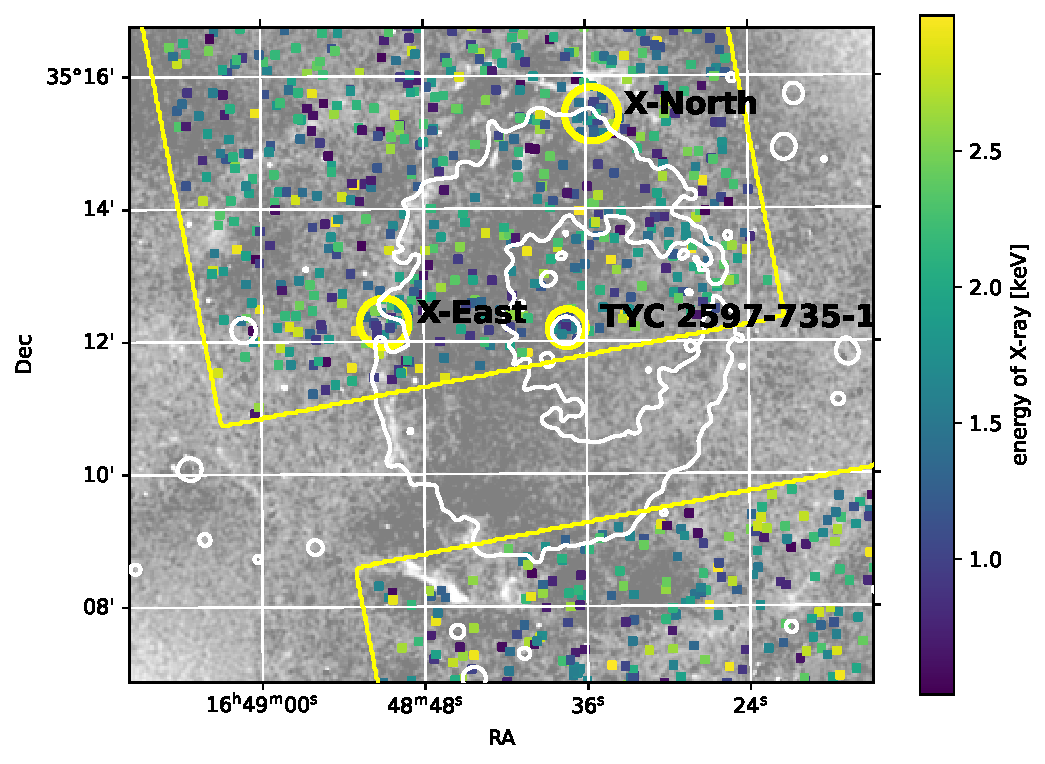
\includegraphics[width=\textwidth]{figures/chandraimage.pdf}
    \caption{X-ray emission around TYC 2597-735-1. The greyscale image shows H$\alpha$ emission and the white contours outline the UV emission. Data for both is taken from \citet{2020Natur.587..387H}, see there for details. The colored squares mark the position of individual X-ray photons, where the color denotes the energy of each particular photon. Only photons in the energy range given on the color bar are shown. Yellow circles mark the position of the three detected sources and their 90\% PSF size, which we use as the extraction region to extract spectra. The thin yellow lines outlines the area covered by Chandra in the observation.}
    \label{fig:chandraimage}
\end{figure*}

\subsection{Source detection}
Because of the large distance, we expect any source associated with TYC 2597-735-1 or its outflow to be absorbed, so we construct a narrow band image in the 1-2~keV range and run a source detection with the CIAO \texttt{wavdetect} task, which convolves the input image with a wavelet, taking the size of the PSF at that image location into account. We bin up the image such that it contains $2.6\times10^4$ pixels in Chandra's field-of-view and set the significant threshold such that we expect no more than one false detection in $10^5$~pixels. That way, any source detected by \texttt{wavdetect} is likely to be real. We find three sources, all of which coincide with UV/optical emission feature. All three sources have similar count rates and similar PSF sizes and thus similar positional uncertainties of about 2\arcsec{}.

We detect a source at the location of TYC 2597-735-1 with (in our narrow band image) $9\pm3$ counts on a background of $1.52\pm0.01$ counts. (The background is known to a high precision because \texttt{wavdetect} determines it over a large area.) Additionally, the probability that any one source randomly overlaps with the known position of TYC 2597-735-1 within the 90\% PSF radius (0.28 arcmin for an energy of 1.5~keV and at the position of TYC 2597-735-1) is only 0.2\%. Thus, we regard this as a highly reliable detection of X-ray emission from TYC 2597-735-1, albeit with large uncertainties on flux and spectral properties due to the small number of counts.

We do detect two other features that are both located just inside the ring of $H\alpha$, one of them is almost due North of TYC 2597-735-1, and the other one to the East (see Fig.~\ref{fig:chandraimage}. The feature to the East has $5\pm2.2$ counts with an estimated background of $1.01\pm0.01$ counts, while the one in the North has $8\pm2.8$ counts with a higher estimated background of $1.96\pm0.01$, because the PSF is wider. Again, the fact that both features are located at a physically meaningful position between the UV emission (white contour Fig.~\ref{fig:chandraimage}) and the bright H$\alpha$ ring (background image in Fig.~\ref{fig:chandraimage}) argues that these are not background fluctuations, but probably very weak sources that are physically associated with the outflow. However, the number of detected photons is low and only deeper X-ray observations will be able to unambiguously confirm these detections.

Given the low number of counts and the size of the Chandra PSF that far away from the aimpoint, all three source are compatible with point sources, but we expect that the latter two sources are probably spatially extended just like the H$\alpha$ and the UV emission is. However, the low count number does not allow us to actually fit the source shape or extent, so we treat them like point sources below. 

\subsection{Source properties}
For all three regions, the detected soft photons are distributed over the observing time; we do not see strong clustering that would indicate a large flare, but given the low count numbers, variability with factors of a few cannot be excluded.

We extract spectra for all three sources using circular extraction regions that encompass 90\% of the PSF at 1.5~keV at the location of the source. A background spectrum is extracted from a large region on the same chip, that is located outside of the UV contours shown in Fig~\ref{fig:chandraimage}. We can describe this background as a flat 

\begin{figure}
    \centering
    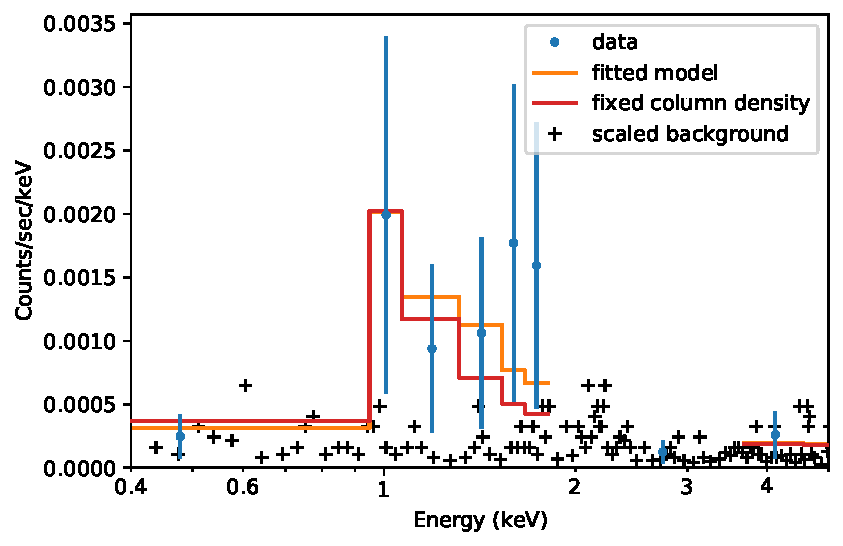
\includegraphics[width=\textwidth]{figures/TYC_spec.pdf}
    \caption{}
    \label{fig:chandraimage}
\end{figure}

\begin{figure}
    \centering
    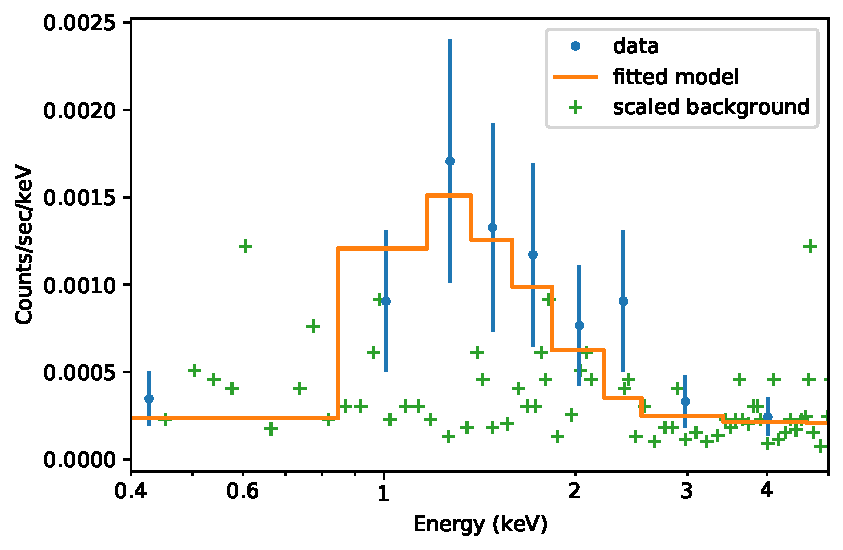
\includegraphics[width=\textwidth]{figures/combined.pdf}
    \caption{}
    \label{fig:chandraimage}
\end{figure}

\section{Discussion}  \label{sec:discussion}

\begin{acknowledgements}
This research has made use of data obtained from the Chandra Data Archive and the Chandra Source Catalog, and software provided by the Chandra X-ray Center (CXC) in the application packages CIAO and Sherpa. 
HMG was supported by the National Aeronautics and Space Administration through Chandra Award Number GO9-20018X issued by the Chandra X-ray Observatory Center, which is operated by the Smithsonian Astrophysical Observatory for and on behalf of the National Aeronautics Space Administration under contract NAS8-03060.
\end{acknowledgements}

\facilities{Chandra/ACIS}

\software{AstroPy \citep{2013A&A...558A..33A,2018AJ....156..123A}, CIAO \citep{2006SPIE.6270E..1VF}, NumPy \citep{van2011numpy,harris2020array}, Matplotlib \citep{Hunter:2007}, Sherpa \citep{2007ASPC..376..543D,doug_burke_2021_4428938}}

\bibliography{bib}{}
\bibliographystyle{aasjournal}

%% This command is needed to show the entire author+affiliation list when
%% the collaboration and author truncation commands are used.  It has to
%% go at the end of the manuscript.
%\allauthors

%% Include this line if you are using the \added, \replaced, \deleted
%% commands to see a summary list of all changes at the end of the article.
%\listofchanges

\end{document}
